\documentclass[a4paper,11pt]{article}
\usepackage[svgnames]{xcolor}
\usepackage{svg}
\usepackage{enumitem}
\usepackage{amsmath}
\usepackage{indentfirst}
\usepackage{listings}
\usepackage{booktabs,colortbl,tabularx}
\usepackage{hyperref}
\usepackage{wrapfig}

\newcolumntype{Y}{>{\arraybackslash}X}
\newcolumntype{C}[1]{>{\centering}p{#1}}
\newcolumntype{R}[1]{>{\raggedright}p{#1}}
\setlength{\arrayrulewidth}{0.5pt}
\setlength{\tabcolsep}{8pt}
\renewcommand{\arraystretch}{1.5}

% \newcolumntype{s}{>{\columncolor[HTML]{AAACED}} p{3cm}}

\arrayrulecolor[HTML]{a0a0a0}
\hypersetup{
    colorlinks,
    citecolor=black,
    filecolor=black,
    linkcolor=black,
    bookmarks=true,
    linkbordercolor=black,
    urlcolor=black
}

\author{Krikun Georgy}
\title{Software Architecture\\Homework 2}
\begin{document}

\begin{titlepage}
\noindent\makebox[\linewidth]{\rule{\paperwidth}{0.4pt}}
{\Large
  \begin{wrapfigure}{l}{40pt}
    \vspace{-12pt}
    \includesvg[width=40pt]{logo_only}
  \end{wrapfigure}
  \hfill
  Innopolis University

  \hfill
  Software Architectures – 2016

  \hfill
  Requirements Specification Document

}

% \end{wrapfigure}

\noindent\makebox[\linewidth]{\rule{\paperwidth}{0.4pt}}\\[60pt]

\begin{flushright}
\huge
{\bfseries{\color{BlueViolet} Lift Controller}}\\[60pt]
\large
Document Version History\\[15pt]
\end{flushright}

\normalsize

\noindent\begin{tabularx}{\textwidth}{|Y|Y|Y|Y|}
  \hline
  Date & Version & Description & Author\\
  \hline
  30/01/2016 & 0.1 & Homework & Krikun G.\\
  \hline
\end{tabularx}

\thispagestyle{empty}
\end{titlepage}

\newpage
\tableofcontents
\newpage
\section{Introduction}
\subsection{Purpose}
This requirements specification document describes the functions and requirements specified for ``Lift Controller''. Also it will illustrate constraints and quality attributes.

This document is primarily intended to be proposed to a customer for its approval and a reference for developing the first version of the system for the development team. But it is written like you know nothing about the lift.

\subsection{Scope}

Lift Controller supposed to use on hardware system, full list of components will describe later. It must controll lift motors, indicators and sensors. Also it must provide safety, call servicing, performance, reliability.

The maximun number of controlling lifts - four lifts per controller, 20 floors. One lift per shaft. All lifts are same numbers of floors. But on common model it could be different.

So at the bottom line, this system is controlled by the people near or inside it. Also guaranteed limited access (could be remote) to the system administration.

A distinctive feature of this device is that it really can kill you, so at least cabin shouldn't smash the floor. Also should be instructions, how to use the lift, maximum load, and other important information, both inside and outside cab. In case of getting stuck in the lift, the cab is provided with a communication service.

\subsection{Functionality}
All lifts, if there're more than one, must be used approximately same. The system can change state (according current) by commands received from command interfaces.

Lift Controller's interfaces:

{\ttfamily
\begin{itemize}
  \item
  Root control panel
  \item
  Floor control buttons
  \item
  Cabin control panel {\itshape\small\color{SlateGray}(could include authentication middleware)}
\end{itemize}
}

A main function is assumes, to transport people and other different goods in vertical direction, up and down. Every floor have a number. To get them designed special shaft, with movable cabin. It is prohibited to access shaft outside the cabin\footnote{%
With the exception of technical staff.}.
On the first and last floors lift must be fully be stopped. On every\footnote{%
Can be limited access. This is about authentication issue.}
floor doors can be opened and closed, depending on the state.

\subsection{Logic}
\label{sub:Logic}
Logic for determining priority of actions may vary. But in common case lift circulates through the mine or stay in static. So we can highlight five\footnote{%
Normal mode is only three of them.}
basic state: \\

\begin{tabular}{ll}
  \hline
  \texttt{Off} & - not powered, in static position.\\
  \texttt{On (Pending)} & - ready to go, powered, but in static.\\
  \texttt{Move} & - in action.\\
  \texttt{Broken} & - powered, but can't function.\\
  \texttt{Drop down} & - emergency case.\\
  \hline
\end{tabular}\\

\section{Glossary}
\label{sec:Glossary}

\begin{description}
  \item[Floor control button(s)] \hfill\\
  Intuitive interface, for call lift. Futher in the text just \texttt{button}. Could be single or double control buttons for lift call in both directions.
  \item[Cabin control panel] \hfill\\
  Complex of buttons, for selection of floor, canceling action, calling services, and management additional functions inside the cabin of lift, like doors managing or cooling system.
  \item[Root control panel] \hfill\\
  Interface (could be remote) for controling state off all lifts. Access to this panel granted only for technical staff.
  \item[Control devices] \hfill\\
  This group of units include buttons, controllers, buses to them, and considered as a self-contained device with declared I/O protocols. Like lift controller, door's motor controller, light controller, etc.
  \item[Control interface (bus access)] \hfill\\
  End-user control points, like floor buttons, cabin's panel, root panel (bus access), power switchers, etc.
  \item[Sensors] \hfill\\
  System units with declared I/O protocols, to provide data feedback about lift system state. It include floor lift sensors, door collision sensor, weight sensors, etc.
  \item[Indicators] \hfill\\
  Output channels for displaying system status. For example lift status indicators (displays current floor), button state indicators (highlight pushed button), sound speakers and so on.
  \item[Authentication middleware] \hfill\\
  Autonomous unit that provides limited access, whatever how. It could be firegerprint access or card key. But should provide I/O standardized connections to other control units.
  \item[Hardware system] \hfill\\
  In this case the system is complex of hardware units that perform the main function of the system. Include:
  \begin{itemize}
    \item \textsc{Power source}
    \item \textsc{Movable mechanisms}
    \item \textsc{Control devices}
    \item \textsc{Control interfaces (bus access)}
    \item \textsc{Sensors system}
    \item \textsc{Indicators complex}
    {\color{SlateGray}\item \textsc{Authentication middlemare}}
  \end{itemize}
  {\color{SlateGray}
  As mentioned earlier system can also include authentication access on some (or all) floors. This middleware can be implemented separately from the system. Here and further colored in gray as not mandatory.}

\end{description}

\section{Product Description}
\label{sec:Product Description}

\subsection{User Roles}
\label{sub:User Roles}


\noindent\begin{tabularx}{\textwidth}{|C{3cm}|Y|}
  \hline
  \rowcolor{LightGray}
  Role & Description\\
  \hline
  \texttt{root, repairer} & Admin user, somebody of technical support. Solve issues from other users, either directly or remotely. But direct access granted only specially for trained staff. For this administrative job could be configurated notifications system.\\[10pt]
  \texttt{common user} & Person who can access to lift directly. Also can call cabin, take the lift and escape.\\[10pt]
  \texttt{\color{SlateGray}authenticated user} & \textmd{\color{SlateGray}In cases when to get access to some floors need access rights.} \\

  \hline
\end{tabularx}

\subsection{High Level Software Features}
\label{sub:High Level Software Features}

\noindent\begin{tabularx}{\textwidth}{|C{4cm}|Y|}
  \hline
  \rowcolor{LightGray}
  High Level Software Functionality & Associated User Histories (US)\\
  \hline
  \texttt{HL-01} & US-xx\\
  \hline
\end{tabularx}

\subsection{User Stories for Functional Requirements}
\label{sub:User Stories for Functional Requirements}

\noindent\begin{tabularx}{\textwidth}{|C{2cm}|Y|}
  \hline
  \rowcolor{LightGray}
  \textbf{US-01} & \textbf{The system diagnostics}\\
  \hline
  Description &
  As a root, I want recognize the system is safe to use.
  \\
  \hline
  Acceptance criteria &
  The lift is powered and ready to go. All sensors functioning properly and detected normal conditions. Lift shafts doors are locked. Root gets feedback.\\
  \hline
  Priority & High\\
  \hline
  Effort & High\\
  \hline
\end{tabularx}\\[15pt]

\noindent\begin{tabularx}{\textwidth}{|C{2cm}|Y|}
  \hline
  \rowcolor{LightGray}
  \textbf{US-02} & \textbf{The system initialization}\\
  \hline
  Description &
  As a user, I want recognize the system is ready to use.
  \\
  \hline
  Acceptance criteria &
  The diagnostic system passed all tests. Outside indicators show that system is ready for use. User find out that can use buttons. \\
  \hline
  Priority & High\\
  \hline
  Effort & Medium\\
  \hline
\end{tabularx}\\[15pt]

\noindent\begin{tabularx}{\textwidth}{|C{2cm}|Y|}
  \hline
  \rowcolor{LightGray}
  \textbf{US-03} & \textbf{Push the call-button}\\
  \hline
  Description &
  As a user, I want call lift for subsequent use.\\
  \hline
  Acceptance criteria &
  Button indicator changes state (turn on). The system accepts request.\\
  \hline
  Priority & High\\
  \hline
  Effort & Low\\
  \hline
\end{tabularx}\\[15pt]

\noindent\begin{tabularx}{\textwidth}{|C{2cm}|Y|}
  \hline
  \rowcolor{LightGray}
  \textbf{US-04} & \textbf{Call command}\\
  \hline
  Description &
  As a user, I want get the lift in soon.
  \\
  \hline
  Acceptance criteria &
  According to the system state criteria could be different:

  When system ready to go or moving in selected direction, lift should start (continue) moving in right direction. Overwise (choosed direction is opposite) call is added to queue, lift continues moving in previous direction, until it finishes the previous task.
  \\
  \hline
  Priority & High\\
  \hline
  Effort & Medium\\
  \hline
\end{tabularx}\\[15pt]

\noindent\begin{tabularx}{\textwidth}{|C{2cm}|Y|}
  \hline
  \rowcolor{LightGray}
  \textbf{US-05} & \textbf{The stop}\\
  \hline
  Description &
  As a user, I want safely get inside the lift.
  \\
  \hline
  Acceptance criteria &
  Side sensors signal that lift present, and located behind the doors, fully stopped. The call-button indicator (or corresponding send-button) turned off. Doors perform open-close cycle.
  \\
  \hline
  Priority & High\\
  \hline
  Effort & High\\
  \hline
\end{tabularx}\\[15pt]

\noindent\begin{tabularx}{\textwidth}{|C{2cm}|Y|}
  \hline
  \rowcolor{LightGray}
  \textbf{US-06} & \textbf{Push the send-button}\\
  \hline
  Description &
  As a user, I want choose the right floor.\\
  \hline
  Acceptance criteria &
  Button indicator changes state (turn on). The system accepts request.
  \\
  \hline
  Priority & High\\
  \hline
  Effort & Low\\
  \hline
\end{tabularx}\\[15pt]

\noindent\begin{tabularx}{\textwidth}{|C{2cm}|Y|}
  \hline
  \rowcolor{LightGray}
  \textbf{US-07} & \textbf{Move command}\\
  \hline
  Description &
  As a user, I want use the lift to get the selected floor.
  \\
  \hline
  Acceptance criteria &
  According to the system state criteria could be different:

  When system ready to go or moving in current direction, lift should start (continue) moving in right direction. If selected not only one floor, last floor in current direction is added to the queue. Overwise (selected floor in opposite direction), lift continues moving in previous direction, until it finishes the previous task.
  \\
  \hline
  Priority & High\\
  \hline
  Effort & Medium\\
  \hline
\end{tabularx}\\[15pt]

\noindent\begin{tabularx}{\textwidth}{|C{2cm}|Y|}
  \hline
  \rowcolor{LightGray}
  \textbf{US-08} & \textbf{The moving}\\
  \hline
  Description &
  As a user, I want safely get selected floor.
  \\
  \hline
  Acceptance criteria &
  Lift normally moves at 1.2 m/sec. In slow mode, before arriving, 0.3 m/sec.
  \\
  \hline
  Priority & High\\
  \hline
  Effort & Low\\
  \hline
\end{tabularx}\\[15pt]

\noindent\begin{tabularx}{\textwidth}{|C{2cm}|Y|}
  \hline
  \rowcolor{LightGray}
  \textbf{US-09} & \textbf{The canceling}\\
  \hline
  Description &
  As a user, I want stop motion at any time.
  \\
  \hline
  Acceptance criteria &
  Lift stops at nearest floor. Doors perform open-close cycle. All last send-commands are canceled.
  \\
  \hline
  Priority & Medium\\
  \hline
  Effort & Low\\
  \hline
\end{tabularx}\\[15pt]

\noindent\begin{tabularx}{\textwidth}{|C{2cm}|Y|}
  \hline
  \rowcolor{LightGray}
  \textbf{US-10} & \textbf{The falling}\\
  \hline
  Description &
  As a user, I want survive in falling lift.
  \\
  \hline
  Acceptance criteria &
  Lift stops with not lethal acceleration. User survive.
  \\
  \hline
  Priority & High\\
  \hline
  Effort & High\\
  \hline
\end{tabularx}\\

\newpage
\subsection{Mock-up of the User Interface}
\label{sub:Mock-up of the User Interface}
  % \vspace{-12pt}
\begin{figure}[h!]
  \begin{wrapfigure}{l}{120pt}
    \vspace{-15pt}
    \includesvg[width=120pt]{user_control}
  \end{wrapfigure}
  Green with yellow buttons indicate choice.
  \begin{enumerate}[label=(\alph*)]
  \item The call-buttons (on floors)
  \item The send-buttons (in the cab)
  \item Root terminal
  \end{enumerate}
  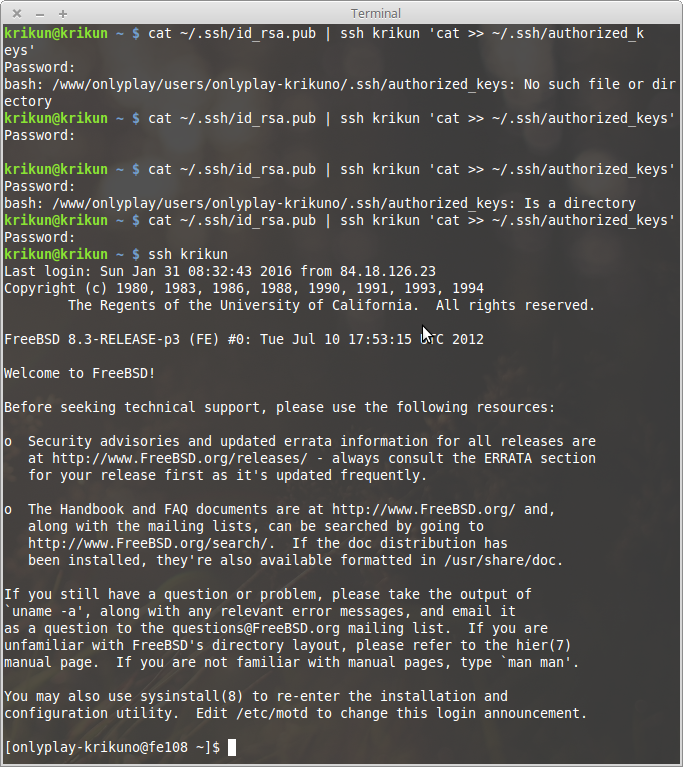
\includegraphics[width=120pt]{root}
\end{figure}
% \vspace{160pt}

\subsection{Non-Functional Requirements / Quality Attributes}
\label{sub:Non-Functional Requirements / Quality Attributes}

\noindent\begin{tabularx}{\textwidth}{|C{2cm}|Y|}
  \hline
  \rowcolor{LightGray}
  \textbf{QA-01} & \textbf{Clear system status}\\
  \hline
  Description &
  The system should clearly show it state.
  \\
  \hline
  Importance & Medium\\
  \hline
  Justification &
  If users don't know system status, they wouldn't use it.
  \\
  \hline
  Measure & Popularity of lift.\\
  \hline
\end{tabularx}\\[15pt]

\noindent\begin{tabularx}{\textwidth}{|C{2cm}|Y|}
  \hline
  \rowcolor{LightGray}
  \textbf{QA-02} & \textbf{Interface usability}\\
  \hline
  Description &
  The system should immediately react on user's actions. (e.g. US-03, US-06)
  \\
  \hline
  Importance & Medium\\
  \hline
  Justification &
  If users don't know system status, they can't use it.
  \\
  \hline
  Measure & Feedback of users, tolerance. Burnt buttons.\\
  \hline
\end{tabularx}\\[15pt]

\subsection{Software Constraints}
\label{sub:Software Constraints}

\noindent\begin{tabularx}{\textwidth}{|C{2cm}|Y|}
  \hline
  \rowcolor{LightGray}
  \textbf{CONS-01} & \textbf{The final stops}\\
  \hline
  Description &
  The system should always stop when arriving at top or bottom.
  \\
  \hline
  Importance & High\\
  \hline
  Justification &
  Overwise possible collisions.
  \\
  \hline
\end{tabularx}\\[15pt]

\noindent\begin{tabularx}{\textwidth}{|C{2cm}|Y|}
  \hline
  \rowcolor{LightGray}
  \textbf{CONS-02} & \textbf{Existing floors}\\
  \hline
  Description &
  The system should moving lift throught give set of floors.
  \\
  \hline
  Importance & High\\
  \hline
  Justification &
  Overwise possible collisions.
  \\
  \hline
\end{tabularx}\\[15pt]

\noindent\begin{tabularx}{\textwidth}{|C{2cm}|Y|}
  \hline
  \rowcolor{LightGray}
  \textbf{CONS-03} & \textbf{Always close the doors}\\
  \hline
  Description &
  The system shouldn't move with open doors.
  \\
  \hline
  Importance & High\\
  \hline
  Justification &
  Overwise possible deaths.
  \\
  \hline
\end{tabularx}
\end{document}
